\documentclass[11pt]{article}

\usepackage[a4paper,margin=25mm]{geometry}
\usepackage{amsmath}
\usepackage{amssymb}
\usepackage{bm}
\usepackage{graphicx}
\usepackage[hidelinks]{hyperref}

\input{macros}

\numberwithin{equation}{section}

\title{Spintronic Methods}
\author{}
\date{\today}

\begin{document}

\maketitle
\tableofcontents

\input{symbols}

\section{Spintronics Concepts}

\subsection{Antiferromagnets}

An antiferromagnet is a magnetic material in which neighboring magnetic moments
prefer an antiparallel arrangement.  The opposing moments can compensate,
giving little or no net magnetization even though the material has long-range
magnetic order.  Its order is therefore described more naturally by a N\'eel
vector than by the net magnetization alone~\cite{xu2023field-free-afm}.

\subsubsection{A-Type Antiferromagnet}

An A-type antiferromagnet consists of ferromagnetic planes stacked
antiferromagnetically: spins within each plane point in the same direction,
all spins in the next plane point in the opposite direction, and the pattern
repeats along the stacking direction.  The word \emph{plane} refers to the
crystallographic planes selected by the exchange interactions in a particular
material.  Figure~\ref{fig:a-type-afm-stacking} chooses the $z$ axis as the
stacking direction as an illustrative convention, not as a universal crystal
orientation.

\paragraph{Source status.}
\textbf{Reference needed.}  This A-type structural classification was supplied
directly for these notes and still needs a dedicated literature reference.

\begin{figure}[htbp]
    \centering
    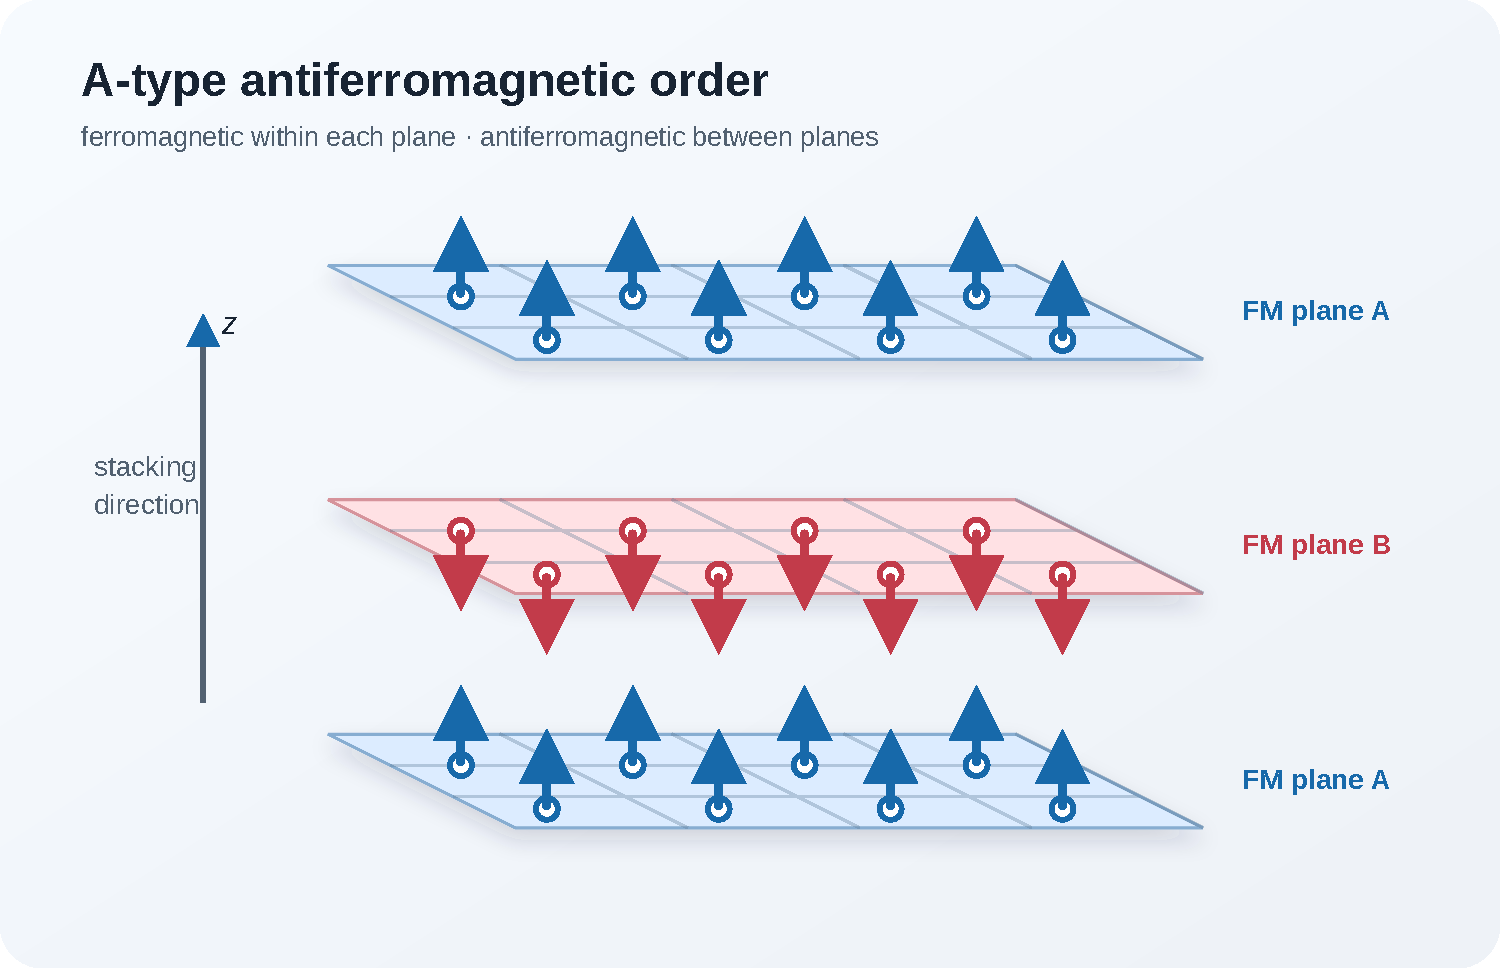
\includegraphics[width=0.92\linewidth]{images/a-type-afm-stacking.pdf}
    \caption{A-type antiferromagnetic stacking: ferromagnetic planes alternate
        in direction.  Original schematic; the physical classification follows
        the provisional description above and therefore shares its
        \textbf{reference-needed} status.}
    \label{fig:a-type-afm-stacking}
\end{figure}

For classical unit spins $\svec_i$, the exchange part of the atomistic
Hamiltonian can be written in the ASTRO sign convention as~\cite{astro-code}
\begin{equation}
    \mathcal{H}_{\mathrm{ex}}
    = \frac{1}{2}\sum_{i\ne j}J_{ij}\,\svec_i\cdot\svec_j.
    \label{eq:a-type-exchange}
\end{equation}
In this convention, A-type order is favored by
\begin{equation}
    J_{\parallel}<0,
    \qquad
    J_{\perp}>0,
    \label{eq:a-type-exchange-signs}
\end{equation}
where $J_{\parallel}$ couples neighbors within a plane and $J_{\perp}$ couples
neighbors in adjacent planes.  Thus the in-plane bonds favor parallel
alignment, whereas the interplane bonds favor antiparallel alignment.  Some
publications place a minus sign in front of the exchange sum; their signs of
$J$ are reversed.  The sign convention and pair counting in
Eq.~\eqref{eq:a-type-exchange} are the same as those used in the full atomistic
Hamiltonian in Eq.~\eqref{eq:atomistic-hamiltonian} and in ASTRO~\cite{astro-code}.

\begin{figure}[htbp]
    \centering
    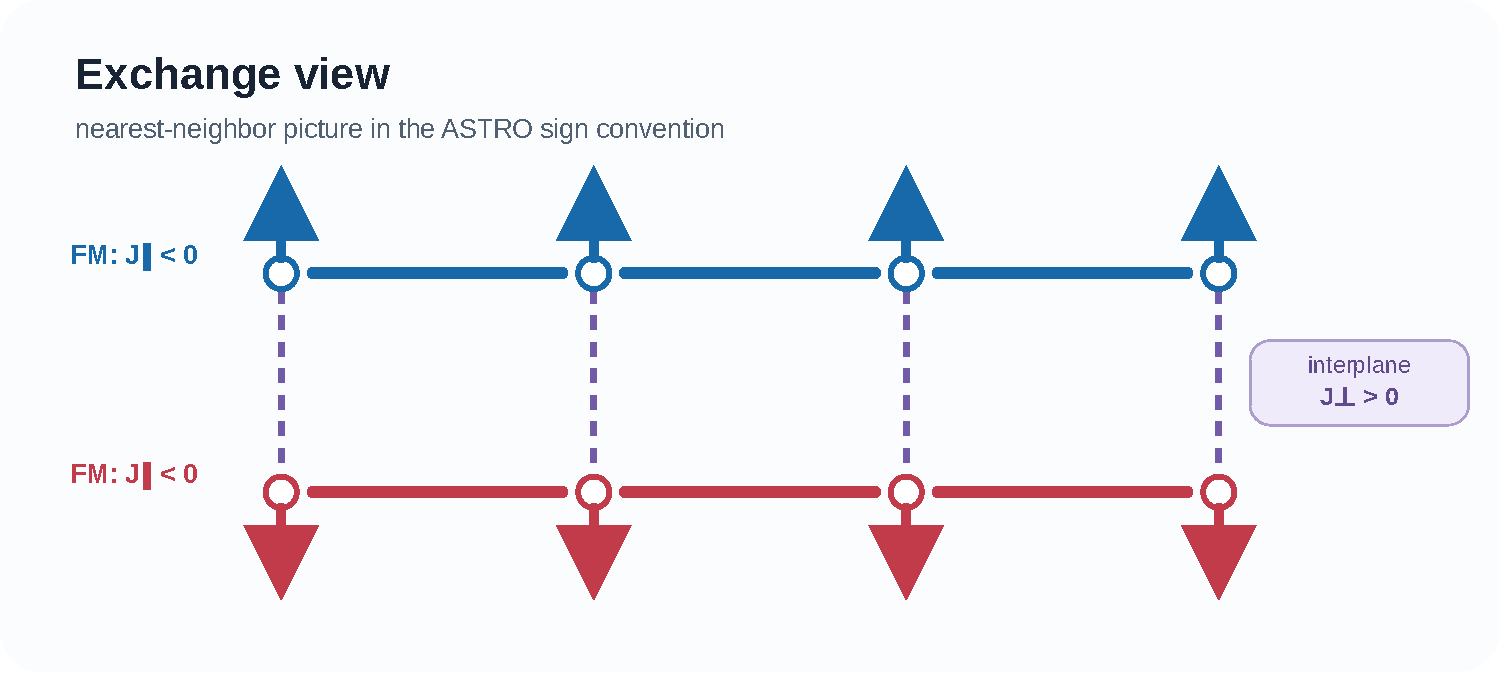
\includegraphics[width=0.95\linewidth]{images/a-type-afm-exchange.pdf}
    \caption{Exchange pattern for A-type order: parallel bonds within a layer
        and antiparallel bonds between layers.  Original schematic based on the
        cited ASTRO exchange-sign convention~\cite{astro-code}; the A-type
        classification itself remains \textbf{reference needed}.}
    \label{fig:a-type-afm-exchange}
\end{figure}

For two equivalent alternating layers with normalized layer magnetizations
$\mathbf{m}_A$ and $\mathbf{m}_B$, define the net and N\'eel order parameters
as~\cite{xu2023field-free-afm}
\begin{equation}
    \mathbf{m}=\frac{\mathbf{m}_A+\mathbf{m}_B}{2},
    \qquad
    \mathbf{n}=\frac{\mathbf{m}_A-\mathbf{m}_B}{2}.
    \label{eq:a-type-order-parameters}
\end{equation}
For an ideal compensated A-type state, these definitions give
\begin{equation}
    \mathbf{m}_B=-\mathbf{m}_A,
    \qquad
    \mathbf{m}=\mathbf{0},
    \qquad
    \lvert\mathbf{n}\rvert=1.
    \label{eq:a-type-compensated-state}
\end{equation}

The defining feature is therefore not simply zero magnetization.  It is the
specific spatial pattern of ferromagnetic order in two directions and
antiferromagnetic alternation in the third.  This distinguishes A-type order
from G-type antiferromagnetism, in which every nearest neighbor is
antiparallel, and C-type order, in which ferromagnetic chains are coupled
antiferromagnetically.  \textbf{Reference needed} for this final classification
comparison.


\section{Symmetries in Spin Systems}

A symmetry operation transforms the spatial coordinates, momenta, spins, and
external fields of a system.  It is a symmetry of a Hamiltonian only when the
transformed Hamiltonian describes the same physical system.  For a unitary
operation $G$ this condition is
\begin{equation}
    G\mathcal{H}G^{-1}=\mathcal{H},
    \label{eq:unitary-symmetry-condition}
\end{equation}
whereas time reversal is antiunitary and also complex-conjugates scalar
coefficients.

\paragraph{Source status.}
\textbf{Reference needed.}  The general time-reversal and spatial-inversion
operator rules in this section are included provisionally because no approved
general reference is currently available.  The mirror rules are supported by
the EE237 notes, the isotropic-exchange example by ASTRO, and the magnetic
parity--time example by Zhang \emph{et al.}, as cited locally below.

\subsection{Polar and Axial Vectors}

Position $\mathbf{r}$, momentum $\mathbf{p}$, electric field $\mathbf{E}$, and
charge-current density $\mathbf{J}$ are polar vectors.  Orbital angular momentum
$\mathbf{L}=\mathbf{r}\times\mathbf{p}$, spin $\mathbf{S}$, magnetization
$\mathbf{M}$, and magnetic field $\mathbf{B}$ are axial vectors.  For an
orthogonal spatial transformation represented by $R$, the two vector classes
transform as
\begin{equation}
    \mathbf{v}'=R\mathbf{v},
    \qquad
    \mathbf{a}'=(\det R)R\mathbf{a},
    \label{eq:polar-axial-transformation}
\end{equation}
where $\mathbf{v}$ is polar and $\mathbf{a}$ is axial.  Thus they transform in
the same way under proper rotations ($\det R=+1$) and differently under mirrors
and inversion ($\det R=-1$)~\cite{ee237-week11}.

The most frequently used transformations are summarized below.  The entries
describe the vector attached to the spatial point after that point has been
mapped by the operation.
\begin{center}
\renewcommand{\arraystretch}{1.25}
\small
\begin{tabular}{|p{0.14\linewidth}|p{0.22\linewidth}|p{0.27\linewidth}|p{0.19\linewidth}|}
    \hline
    Operation & $\mathbf{r},\mathbf{p}$ & $\mathbf{S},\mathbf{M}$ &
    $\mathbf{E},\mathbf{B}$ \\
    \hline
    Time reversal $\mathcal{T}$ &
    $\mathbf{r}\to\mathbf{r}$, $\mathbf{p}\to-\mathbf{p}$ &
    $\mathbf{S},\mathbf{M}\to-\mathbf{S},-\mathbf{M}$ &
    $\mathbf{E}\to\mathbf{E}$, $\mathbf{B}\to-\mathbf{B}$ \\
    \hline
    Inversion $\mathcal{P}$ &
    $\mathbf{r},\mathbf{p}\to-\mathbf{r},-\mathbf{p}$ &
    $\mathbf{S},\mathbf{M}\to\mathbf{S},\mathbf{M}$ &
    $\mathbf{E}\to-\mathbf{E}$, $\mathbf{B}\to\mathbf{B}$ \\
    \hline
    Mirror $\mathcal{M}_{\mathbf{n}}$ &
    $\mathbf{v}\to\mathbf{v}-2\mathbf{n}(\mathbf{n}\cdot\mathbf{v})$ &
    $\mathbf{a}\to-\mathbf{a}+2\mathbf{n}(\mathbf{n}\cdot\mathbf{a})$ &
    polar $\mathbf{E}$; axial $\mathbf{B}$ \\
    \hline
\end{tabular}
\end{center}

\subsection{Time-Reversal Symmetry}

Time reversal changes $t\to-t$ and reverses momenta and angular momenta.  Spin
is an intrinsic angular momentum, so
\begin{equation}
    \mathcal{T}\mathbf{S}\mathcal{T}^{-1}=-\mathbf{S},
    \qquad
    \mathcal{T}i\mathcal{T}^{-1}=-i.
    \label{eq:time-reversal-spin}
\end{equation}
For a classical magnetization trajectory, the corresponding transformed
trajectory is
\begin{equation}
    \mathbf{m}_{\mathcal{T}}(t)=-\mathbf{m}(-t).
    \label{eq:time-reversed-magnetization}
\end{equation}
A magnetic state can therefore break time-reversal symmetry even when its
nonmagnetic crystal structure does not.  A fixed applied magnetic field, a
fixed current, damping, or another nonequilibrium drive must not be silently
left unchanged when testing time reversal; these time-odd or irreversible
ingredients generally prevent the driven equation from being
time-reversal-invariant.

\paragraph{Source status.}
\textbf{Reference needed.}  Equations~\eqref{eq:time-reversal-spin} and
\eqref{eq:time-reversed-magnetization}, and the general invariance statement
above, still need an approved reference.

\subsection{Parity or Spatial-Inversion Symmetry}

Here parity means full spatial inversion,
\begin{equation}
    \mathcal{P}:\quad \mathbf{r}\to-\mathbf{r}.
    \label{eq:spatial-inversion}
\end{equation}
Because spin is axial, inversion moves a spin to the inverted site without
reversing its direction.  For a spin texture this gives
\begin{equation}
    \mathbf{S}_{\mathcal{P}}(\mathbf{r})
    =\mathbf{S}(-\mathbf{r}).
    \label{eq:inverted-spin-texture}
\end{equation}
The structure has inversion symmetry only when the inverted sites, chemical
species, interactions, and spin pattern reproduce the original structure.
This is distinct from particle-exchange symmetry.  In non-Hermitian coupled-mode
models the symbol $\mathcal{P}$ may instead denote exchange of two subsystems;
its meaning must therefore be stated explicitly.

\paragraph{Source status.}
\textbf{Reference needed.}  Equations~\eqref{eq:spatial-inversion} and
\eqref{eq:inverted-spin-texture}, including the axial-spin convention under
inversion, still need an approved general reference.

\subsection{Mirror Symmetry}

A mirror with unit normal $\mathbf{n}$ reverses the perpendicular component of
a polar vector.  An axial vector behaves oppositely: its components parallel to
the mirror plane reverse, while its perpendicular component is unchanged
according to Eq.~\eqref{eq:polar-axial-transformation}~\cite{ee237-week11}.
For the $xy$ mirror,
\begin{equation}
    (v_x,v_y,v_z)\to(v_x,v_y,-v_z),
    \qquad
    (S_x,S_y,S_z)\to(-S_x,-S_y,S_z).
    \label{eq:xy-mirror-polar-axial}
\end{equation}
The transformed lattice and every axial spin must both be compared with the
original magnetic structure.  A lattice may therefore possess a mirror plane
that is broken by its magnetic order.

\subsection{Spin-Rotation Symmetry}

Spatial rotations move the lattice, whereas spin rotations act in spin space.
For the isotropic exchange Hamiltonian used in ASTRO,
\begin{equation}
    \mathcal{H}_{\mathrm{ex}}
    =\frac{1}{2}\sum_{i\ne j}J_{ij}\,\mathbf{S}_i\cdot\mathbf{S}_j,
    \label{eq:symmetry-isotropic-exchange}
\end{equation}
a common spin rotation $R_s$ leaves every dot product unchanged:
\begin{equation}
    (R_s\mathbf{S}_i)\cdot(R_s\mathbf{S}_j)
    =\mathbf{S}_i\cdot\mathbf{S}_j.
    \label{eq:global-spin-rotation}
\end{equation}
The exchange term consequently has global spin-rotation symmetry when the
couplings $J_{ij}$ do not depend on spin direction~\cite{astro-code}.  Magnetic
anisotropy, Dzyaloshinskii--Moriya interaction, dipolar coupling, an applied
field, or another spin--orbit-coupled term can reduce this continuous symmetry
to the subset of joint spatial and spin operations that preserves the complete
Hamiltonian.

\subsection{Combined Parity--Time Symmetry in a Two-Sublattice Magnet}

For the two-sublattice order parameters defined in
Eq.~\eqref{eq:a-type-order-parameters}, suppose that inversion exchanges
sublattices $A$ and $B$.  Since inversion does not reverse an axial spin,
whereas time reversal does, their actions are
\begin{equation}
\begin{array}{c|cc}
    & \mathbf{m} & \mathbf{n} \\
    \hline
    \mathcal{P} & \mathbf{m} & -\mathbf{n} \\
    \mathcal{T} & -\mathbf{m} & -\mathbf{n} \\
    \mathcal{P}\mathcal{T} & -\mathbf{m} & \mathbf{n}
\end{array}
    \label{eq:pt-order-parameters}
\end{equation}
Thus a compensated antiferromagnetic pattern can be invariant under the
combined operation even when it is not invariant under $\mathcal{P}$ or
$\mathcal{T}$ separately.  In a different use of parity, Zhang \emph{et al.}
define $\mathcal{P}$ as interchange of two coupled ferrimagnetic layers and
obtain parity--time-symmetric N\'eel-vector dynamics at angular-momentum
compensation~\cite{zhang2024nonhermitian}.  These two meanings should not be
conflated.

\paragraph{Source status.}
\textbf{Reference needed.}  Equation~\eqref{eq:pt-order-parameters} is a direct
derivation from the provisional general transformation rules above.  The cited
paper supports only the separate coupled-layer example.

\subsection{Practical Symmetry Test}

To test a proposed symmetry of a spin model:
\begin{enumerate}
    \item map every position and sublattice label;
    \item transform spin as an axial vector and reverse it additionally under
        time reversal;
    \item transform external fields, currents, and boundary conditions;
    \item rebuild every Hamiltonian or dynamical term with the transformed
        quantities; and
    \item compare the complete transformed model and magnetic pattern with the
        originals.
\end{enumerate}
Checking only the atomic lattice or only the spin arrows is insufficient for a
magnetic symmetry.

\paragraph{Source status.}
\textbf{Reference needed.}  The general five-step test is a provisional
pedagogical synthesis and still needs an approved reference.


\section{Representative Material Parameter Sets}

The values below reproduce particular numerical models from papers and
repository implementations authored or coauthored by Zhifeng Zhu.  They are
model-specific parameter sets rather than universal material constants.  In
particular, quantities associated with a heavy-metal layer, spin polarization,
device geometry, or numerical integration are identified separately from
intrinsic magnetic parameters.  Fixed-length unit vectors are used in all three
source-model families summarized here.

\subsection{Property of Heavy Metal}

The spin-Hall angle belongs to the heavy-metal spin-current source and is not
specific to a ferromagnetic, ferrimagnetic, or antiferromagnetic target layer.
For the signed representative values in Table~\ref{tab:heavy-metal-properties},
we use
$\vect{J}_{\mathrm{s}}=\theta_{\mathrm{SH}}\,
\vect{\sigma}\times\vect{J}_{\mathrm{c}}$ and choose Pt as the positive
reference; Ta and W then have negative signs~\cite{sot-stt-compact-model,
liu2012ta-spin-hall,pai2012w-spin-hall}.  Reversing the current, layer-normal,
or spin-polarization convention requires a corresponding sign change in the
torque implementation.

\begin{table}[htbp]
    \centering
    \small
    \renewcommand{\arraystretch}{1.15}
    \begin{tabular}{p{0.16\linewidth}p{0.31\linewidth}p{0.42\linewidth}}
        \hline
        Property & Value & Evidence and qualification \\
        \hline
        Pt spin-Hall angle
            & $+0.07$
            & Representative literature value quoted by Liu et al. and Pai et
              al.; defines the positive reference sign \\
        High-resistivity $\beta$-Ta spin-Hall angle
            & $-0.12$ to $-0.15$
            & Consistent magnitudes from ST-FMR, perpendicular switching, and
              three-terminal switching \\
        High-resistivity $\beta$-W spin-Hall angle
            & $-0.30\pm0.02$ (ST-FMR);
              $-0.33\pm0.06$ (switching)
            & Negative sign verified relative to Pt; the ST-FMR value is a
              lower bound if spin diffusion suppresses the measured torque \\
        Heavy-metal resistivity
            & $\rho_{\mathrm{HM}}=200\times10^{-8}\ \Omega\,\mathrm{m}$
            & Representative Ta/W value from the compact model;
              $\rho_{\mathrm{HM}}=200\ \mu\Omega\,\mathrm{cm}$ \\
        \hline
    \end{tabular}
    \caption{Representative properties of Pt, $\beta$-Ta, and $\beta$-W
    heavy metals~\cite{sot-stt-compact-model,liu2012ta-spin-hall,
    pai2012w-spin-hall}.}
    \label{tab:heavy-metal-properties}
\end{table}

These values are not universal elemental constants.  In particular, Pai et al.
find that W changes strongly with film phase and resistivity: a mixed
$\alpha$/$\beta$ film gives $\lvert\theta_{\mathrm{SH}}\rvert=0.18\pm0.02$,
whereas their predominantly $\alpha$-W film gives only the upper bound
$\lvert\theta_{\mathrm{SH}}\rvert<0.07$~\cite{pai2012w-spin-hall}.  The
material-specific tables below omit $\theta_{\mathrm{SH}}$; select a value from
the heavy-metal source and sign convention used by the model.

The compact-model README compares reported resistivities of
$190\ \mu\Omega\,\mathrm{cm}$ for Ta and $170$--$260\ \mu\Omega\,\mathrm{cm}$
for W, then uses the representative value
$\rho_{\mathrm{HM}}=200\ \mu\Omega\,\mathrm{cm}$~\cite{sot-stt-compact-model}.

\subsection{Ferromagnet: CoFeB}

The CoFeB free layer is represented by a one-sublattice macrospin LLGS model
with perpendicular anisotropy.  The anisotropy field and saturation magnetization
below are the defaults of the SOT/STT compact model; the remaining magnetic and
drive parameters come from the model of Zhang et
al.~\cite{sot-stt-compact-model,zhang2024revisiting}.  The compact-model
parameter named \texttt{Hk} is a flux-density quantity in tesla.  Its
corresponding $\vect{H}$ field in $\mathrm{A\,m^{-1}}$ is obtained by dividing
by $\mu_0$.

\begin{table}[htbp]
    \centering
    \small
    \renewcommand{\arraystretch}{1.15}
    \begin{tabular}{p{0.25\linewidth}p{0.28\linewidth}p{0.36\linewidth}}
        \hline
        Quantity & Value & Role or convention \\
        \hline
        Uniaxial anisotropy field
            & $B_k=1.5\ \mathrm{T}$
            & Compact-model parameter \texttt{Hk};
              $H_k\approx1.19\times10^6\ \mathrm{A\,m^{-1}}$ \\
        Saturation magnetization
            & $M_s=1000\ \mathrm{emu\,cm^{-3}}$
            & $M_s=1.00\times10^6\ \mathrm{A\,m^{-1}}$;
              $\mu_0M_s\approx1.26\ \mathrm{T}$ \\
        Gilbert damping
            & $\alpha=0.02$
            & Magnetic model parameter \\
        \hline
    \end{tabular}
    \caption{Selected CoFeB macrospin parameters from the SOT/STT compact model
    and Zhang et al.~\cite{sot-stt-compact-model,zhang2024revisiting}.}
    \label{tab:cofeb-parameters}
\end{table}

\paragraph{Parameter justification.}
Based on Nat. Mater. \textbf{9}, 721 (2010).,
$H_{\mathrm{an}}=2(K_{\mathrm{bulk}}+K_i/t_{\mathrm{FL}})/M_s$ with
$K_{\mathrm{bulk}}=2.245\times10^5\ \mathrm{J\,m^{-3}}$,
$K_i=1.286\times10^{-3}\ \mathrm{J\,m^{-2}}$,
$M_s=1.58\ \mathrm{T}=1257\ \mathrm{emu\,cm^{-3}}$, when we use
$t_{\mathrm{FL}}=1.2\ \mathrm{nm}$, it gives $H_{\mathrm{an}}=2.06\ \mathrm{T}$.
Here we approximate $M_s=1000\ \mathrm{emu\,cm^{-3}}$,
$H_k=1.5\ \mathrm{T}$~\cite{sot-stt-compact-model}.

\subsection{Ferrimagnet: GdFeCo}

Zhang et al. use a random two-dimensional atomistic
$(\mathrm{FeCo})_{1-x}\mathrm{Gd}_x$ lattice driven by damping-like STT,
whereas Zhu et al. use a one-dimensional atomistic GdFeCo model driven by
SOT~\cite{zhang2022spatially,zhu2020terahertz}.  Both are fixed-length LLG or
LLGS models.  The 2022 paper states that its parameters are otherwise the same
as those in the 2020 paper, but replaces the single exchange coefficient with
three bond-specific values.  Table~\ref{tab:gdfeco-parameters} therefore keeps
the two published exchange parameterizations separately rather than selecting
or averaging them.

\begin{table}[htbp]
    \centering
    \small
    \renewcommand{\arraystretch}{1.15}
    \begin{tabular}{p{0.19\linewidth}p{0.31\linewidth}p{0.31\linewidth}}
        \hline
        Quantity & Zhu et al. (2020) & Zhang et al. (2022) \\
        \hline
        Spatial model
            & 1D atomistic lattice with lattice constant $d=0.4\ \mathrm{nm}$;
              strip length and width are $400$ and $40\ \mathrm{nm}$
            & Random 2D square lattice; each interior site has four nearest
              neighbors; the main phase diagrams use 100 atoms \\
        Exchange
            & $A_{\mathrm{ex}}=+3\ \mathrm{meV}
              =+4.8065\times10^{-22}\ \mathrm{J}$
            & $A_{\mathrm{Gd-Gd}}=-1.26\times10^{-21}\ \mathrm{J}$;
              $A_{\mathrm{FeCo-FeCo}}=-2.83\times10^{-21}\ \mathrm{J}$;
              $A_{\mathrm{FeCo-Gd}}=+1.09\times10^{-21}\ \mathrm{J}$ \\
        Perpendicular anisotropy
            & $K_{\mathrm{TM}}=K_{\mathrm{RE}}=0.04\ \mathrm{meV}$
            & same as Zhu et al. (2020) \\
        Hard-axis anisotropy
            & $\kappa_{\mathrm{TM}}=\kappa_{\mathrm{RE}}=0.2\ \mu\mathrm{eV}$
            & Not included in the stated Hamiltonian \\
        DMI
            & $D=0.128\ \mathrm{meV}$
            & Not included in the stated Hamiltonian \\
        Gilbert damping
            & $\alpha_{\mathrm{TM}}=\alpha_{\mathrm{RE}}=0.015$
            & same as Zhu et al. (2020) \\
        Land\'e factors
            & $g_{\mathrm{TM}}=2.2$; $g_{\mathrm{RE}}=2.0$
            & same as Zhu et al. (2020) \\
        Sublattice magnetizations
            & $M_{s,\mathrm{TM}}=1149\ \mathrm{kA\,m^{-1}}$;
              $M_{s,\mathrm{RE}}=1012\ \mathrm{kA\,m^{-1}}$ at
              $T=300\ \mathrm{K}$
            & same as Zhu et al. (2020) \\
        Ferrimagnet thickness
            & $t_{\mathrm{FiM}}=0.4\ \mathrm{nm}$
            & same as Zhu et al. (2020) \\
        Drive parameter
            & Spin-Hall angle $\theta_{\mathrm{SH}}=0.2$; field-like to
              damping-like ratio $\beta$ is varied rather than fixed in the
              baseline list
            & STT efficiency $\eta$ is introduced but no numerical value is
              stated \\
        Compensation composition
            & Not stated as a composition in the parameter block
            & $x_{\mathrm{MC}}=0.23$;
              $x_{\mathrm{AMC}}=0.21$ \\
        \hline
    \end{tabular}
    \caption{Atomistic GdFeCo parameter sets retained in their native model
    conventions~\cite{zhu2020terahertz,zhang2022spatially}.}
    \label{tab:gdfeco-parameters}
\end{table}

The exchange values are deliberately not converted into a single common
coefficient.  The 2020 value belongs to a one-dimensional nearest-neighbor
Hamiltonian, while the 2022 values distinguish the chemical identity of each
bond in a random two-dimensional alloy.  Their lattice topology and bond
statistics must be retained with the numerical values when either set is used.

\subsection{Noncollinear Antiferromagnet:
\texorpdfstring{Mn$_3$Sn}{Mn3Sn}}

The three-sublattice macrospin switching model of Xu et al. and the later
spatially resolved atomistic domain-wall model use the same magnetic moment,
DMI, anisotropy, damping, and spin-Hall angle, but different exchange
coefficients~\cite{xu2024mn3sn,xu2025mn3sn-domain-wall}.  The values must
therefore remain attached to their model and interaction convention.  Both
Hamiltonians take positive $A$ to favor antiparallel alignment, and the
crystalline easy axes point toward the nearest Sn atoms.  The atomistic
domain-wall paper additionally states that its positive $D$ favors clockwise
order.

\begin{table}[htbp]
    \centering
    \small
    \renewcommand{\arraystretch}{1.15}
    \begin{tabular}{p{0.23\linewidth}p{0.29\linewidth}p{0.38\linewidth}}
        \hline
        Quantity & Value & Model scope or convention \\
        \hline
        Mn moment
            & $m_s=3\mu_B$
            & Per Mn site in both models \\
        Nearest-neighbor exchange
            & $A=17.53\ \mathrm{meV}$
            & Three-sublattice macrospin switching model \\
        Nearest-neighbor exchange
            & $A=9\ \mathrm{meV}$
            & Spatial atomistic domain-wall model \\
        DMI coefficient
            & $D=0.833\ \mathrm{meV}$
            & Same-layer interaction in both models \\
        Crystalline anisotropy
            & $K=0.196\ \mathrm{meV}$
            & Single-site Hamiltonian coefficient in both models \\
        Gilbert damping
            & $\alpha=0.003$
            & Same in both fixed-length models \\
        Unit-cell volume
            & $V_{\mathrm{cell}}=0.3778\ \mathrm{nm^3}$
            & Macrospin model; $M_s=6m_s/V_{\mathrm{cell}}
              \approx4.42\times10^5\ \mathrm{A\,m^{-1}}$ \\
        Mn$_3$Sn thickness
            & $d=30\ \mathrm{nm}$
            & Macrospin SOT model geometry \\
        Time step
            & $\Delta t=5\ \mathrm{fs}$
            & Fourth-order Runge--Kutta macrospin integration \\
        Nanoribbon length
            & $5.7\,\mu\mathrm{m}$
            & Spatial atomistic domain-wall model geometry \\
        \hline
    \end{tabular}
    \caption{Mn$_3$Sn parameter sets used in the macrospin switching and
    atomistic domain-wall models~\cite{xu2024mn3sn,xu2025mn3sn-domain-wall}.}
    \label{tab:mn3sn-parameters}
\end{table}

The Mn$_3$Sn entries are not by themselves a complete crystallographic
simulation specification: a reproducible atomistic calculation must also retain
the source model's lattice, site mapping, bond list, DMI-vector orientations,
boundary conditions, and pair-counting convention.


\section{Spin Hamiltonians}
\input{sections/hamiltonian}
\subsection{Macrospin Effective Fields}

\paragraph{Field convention.}
For a fixed-length macrospin with normalized magnetization $\mvec$, let $w$
denote the magnetic energy density in $\mathrm{J\,m^{-3}}$.  The effective
magnetic field and the corresponding effective flux density are~\cite{ee237-week5}
\begin{equation}
    \Heff
    =-\frac{1}{\mu_0\Ms}\frac{\partial w}{\partial\mvec},
    \qquad
    \vect{B}_{\mathrm{eff}}=\mu_0\Heff.
    \label{eq:macrospin-effective-field}
\end{equation}
Thus, an LLG equation written with $\gamma_0=\mu_0\abs{\gamma}$ uses
$\Heff$ in $\mathrm{A\,m^{-1}}$, whereas one written with
$\abs{\gamma}$ uses $\vect{B}_{\mathrm{eff}}$ in tesla.  The two
conventions are physically equivalent but their field variables must not be
mixed.

Unless stated otherwise, $K_u$ and $A_{12}$ are energy densities in
$\mathrm{J\,m^{-3}}$.  The interfacial $K_i$ in the combination
$K_{\mathrm{bulk}}+K_i/t_{\mathrm{FM}}$ is instead in
$\mathrm{J\,m^{-2}}$, and every saturation magnetization is in
$\mathrm{A\,m^{-1}}$.  The tensors $\mathsf{N}$ and $\mathsf{K}_{fp}$ are
dimensionless.

\subsubsection{One-Sublattice Model}

\paragraph{Energy density and field decomposition.}
For uniaxial anisotropy with easy axis $\unitvect{u}$, a dimensionless
symmetric demagnetization tensor $\mathsf{N}$, an applied field
$\vect{H}_{\mathrm{ext}}$, and a dipolar field $\vect{H}_{\mathrm{dip}}$
produced by another magnetic body, use the uniaxial-anisotropy convention
from slides 13--14 of the EE237 Week 5 lecture notes~\cite{ee237-week5} and
take
\begin{equation}
    w_1
    =K_u\left[1-\bigl(\mvec\cdot\unitvect{u}\bigr)^2\right]
    +\frac{\mu_0\Ms^2}{2}\mvec\cdot\mathsf{N}\mvec
    -\mu_0\Ms\mvec\cdot
    \bigl(\vect{H}_{\mathrm{ext}}+\vect{H}_{\mathrm{dip}}\bigr).
    \label{eq:one-sublattice-energy}
\end{equation}

\paragraph{External field.}
The part of the final term in Eq.~\eqref{eq:one-sublattice-energy} that is
proportional to $\vect{H}_{\mathrm{ext}}$ is the Zeeman coupling to the
applied field.  Its derivative contributes $\vect{H}_{\mathrm{ext}}$ directly
to $\Heff$~\cite{ee237-week5}.

\paragraph{Uniaxial anisotropy field.}
Equation~\eqref{eq:macrospin-effective-field} gives~\cite{ee237-week5}
\begin{equation}
    \vect{H}_{\mathrm{an}}
    =\frac{2K_u}{\mu_0\Ms}
    \bigl(\mvec\cdot\unitvect{u}\bigr)\unitvect{u},
    \qquad
    \vect{B}_{\mathrm{an}}
    =\frac{2K_u}{\Ms}
    \bigl(\mvec\cdot\unitvect{u}\bigr)\unitvect{u}.
    \label{eq:macrospin-anisotropy-field}
\end{equation}
For $\unitvect{u}=\unitvect{z}$, the anisotropy term reduces to
$K_u(1-m_z^2)=K_u\sin^2\theta$, as on slide 13. Near $m_z=1$, slide 14
therefore gives $H_{\mathrm{an},z}=2K_u/(\mu_0\Ms)$.
For a thin film with bulk and interfacial uniaxial anisotropy,
$K_u=K_{\mathrm{bulk}}+K_i/t_{\mathrm{FM}}$.

\paragraph{Demagnetization field.}
Slide 21 of the same notes writes the demagnetization self-energy
as~\cite{ee237-week5}
\begin{align}
    E_{\mathrm{demag}}
     & =-\frac{\mu_0}{2}\int_V
    \vect{M}(\vect{r})\cdot\vect{H}_{\mathrm{demag}}(\vect{r})
    \,\dd^3r,
    \label{eq:macrospin-demag-energy-integral}                 \\
    w_{\mathrm{demag}}
     & =-\frac{\mu_0}{2}\vect{M}\cdot\vect{H}_{\mathrm{demag}}
    =\frac{\mu_0\Ms^2}{2}\mvec\cdot\mathsf{N}\mvec
    \quad\text{(uniform macrospin)}.
    \label{eq:macrospin-demag-energy-density}
\end{align}
The factor $1/2$ avoids double counting the magnet's self-interaction.
Equation~\eqref{eq:macrospin-effective-field} gives
\begin{equation}
    \vect{H}_{\mathrm{demag}}
    =-\Ms\mathsf{N}\mvec,
    \qquad
    \vect{B}_{\mathrm{demag}}
    =-\mu_0\Ms\mathsf{N}\mvec.
    \label{eq:macrospin-demag-field}
\end{equation}
For principal axes,
$\mathsf{N}=\operatorname{diag}(N_x,N_y,N_z)$ and
$N_x+N_y+N_z=1$.

\paragraph{Dipolar field.}
Let a pinned macrospin have volume $V_p$, saturation magnetization
$M_{\mathrm{s},p}$, and direction $\mvec_p$, so its magnetic moment is
$\vect{\mu}_p=V_pM_{\mathrm{s},p}\mvec_p$.
In the point-dipole approximation, at displacement
$\vect{r}=r\unitvect{r}$ from the pinned layer to the free layer, slide 22
gives the dipole formula~\cite{ee237-week5}.  The slide denotes it by
$\vect{H}_i$, but its factor $\mu_0$ makes it a flux density in tesla;
therefore, in the convention of this document,
\begin{align}
    \vect{B}_{\mathrm{dip}}
     & =\frac{\mu_0}{4\pi r^3}
    \left[3\bigl(\vect{\mu}_p\cdot\unitvect{r}\bigr)\unitvect{r}
        -\vect{\mu}_p\right]
    =\mu_0\vect{H}_{\mathrm{dip}},
    \label{eq:macrospin-dipole-flux-density}
\end{align}

\paragraph{Thermal field.}
Following Eq.~(4) of Zhu et al.~\cite{zhu2019voltage}, write the sampled
thermal field as
\begin{align}
    \vect{B}_{\mathrm{th}}
    =\mu_0\Hth
     & =\mathcal{N}_1(0,u_B)\unitvect{x}
    +\mathcal{N}_2(0,u_B)\unitvect{y}
    +\mathcal{N}_3(0,u_B)\unitvect{z},
    \label{eq:thermal-field-discrete}              \\
    u_B
     & =\sqrt{\frac{2\alpha\kB T}
            {V_{\mathrm{FL}}\Ms\abs{\gamma}
                \left(1+\alpha^2\right)\Delta t}}.
    \label{eq:thermal-field-standard-deviation}
\end{align}
Here the $\mathcal{N}_i(0,u_B)$ are independent normal random variables with
zero mean and standard deviation $u_B$, $V_{\mathrm{FL}}$ is the free-layer
volume, and $\Delta t$ is the duration over which a sampled field is held
constant.  With $\abs{\gamma}$ in $\mathrm{rad\,s^{-1}\,T^{-1}}$ and $\Ms$ in
$\mathrm{A\,m^{-1}}$, $u_B$ is in tesla; the corresponding $\vect{H}$-field
standard deviation is $u_H=u_B/\mu_0$.

The source uses independent samples over
$\Delta t=5\,\mathrm{ps}$~\cite{zhu2019voltage}.  When adopting another
integration interval or LLG convention, recompute the noise amplitude
consistently rather than reusing that numerical value.

\paragraph{Total field.}
The total one-sublattice field, with the stochastic field added after taking
the energy derivative, is~\cite{ode-llg-code}
\begin{equation}
    \Heff
    =\vect{H}_{\mathrm{ext}}
    +\vect{H}_{\mathrm{an}}
    +\vect{H}_{\mathrm{demag}}
    +\vect{H}_{\mathrm{dip}}
    +\Hth.
    \label{eq:one-sublattice-total-field}
\end{equation}
Spin-transfer and spin--orbit torques are nonconservative and are not part of
the energy derivative in Eq.~\eqref{eq:macrospin-effective-field}.

\paragraph{Implementation mapping.}
The current one-sublattice \texttt{ODE\_LLG\_integral} implementation stores
flux-density quantities in tesla~\cite{ode-llg-code}.  Its
\texttt{field\_eta.m} evaluates the following expressions, where its input
named \texttt{Hk} is $B_k$:
\begin{align*}
    \vect{B}_{\mathrm{an}}
     & =B_k m_y\unitvect{y} \quad\text{(IMA)},
     &
    \vect{B}_{\mathrm{an}}
     & =B_k m_z\unitvect{z} \quad\text{(PMA)},      \\
    \vect{B}_{\mathrm{demag}}
     & =-\mu_0\Ms\mathsf{N}\mvec,
     &
    \vect{B}_{\mathrm{dip}}
     & =\mu_0\mathsf{K}_{12}\Ms\mvec_{\mathrm{PL}},
\end{align*}
after converting the input $\Ms$ from $\mathrm{emu\,cm^{-3}}$ to
$\mathrm{A\,m^{-1}}$.  It sums these with the applied and thermal fields.

\subsubsection{Two-Sublattice Collinear Model}

\paragraph{Inter-sublattice exchange field.}
Let $\mvec_1$ and $\mvec_2$ be separately normalized sublattice
magnetizations with saturation magnetizations $M_{\mathrm{s},1}$ and
$M_{\mathrm{s},2}$.  The exchange-energy density convention used by the
two-sublattice ferrimagnetic macrospin model of Yuan et
al.~\cite{yuan2023thermal} is
\begin{equation}
    w_{\mathrm{ex},12}=A_{12}\mvec_1\cdot\mvec_2,
    \qquad A_{12}>0,
    \label{eq:two-sublattice-exchange-energy}
\end{equation}
Applying
$\vect{H}_{\mathrm{ex},i}=-(\mu_0M_{\mathrm{s},i})^{-1}
    \partial w_{\mathrm{ex},12}/\partial\mvec_i$ yields, for $j\ne i$,
\begin{equation}
    \vect{H}_{\mathrm{ex},i}
    =-\frac{A_{12}}{\mu_0M_{\mathrm{s},i}}\mvec_j,
    \qquad
    \vect{B}_{\mathrm{ex},i}
    =-\frac{A_{12}}{M_{\mathrm{s},i}}\mvec_j.
    \label{eq:two-sublattice-exchange-field}
\end{equation}

Only the exchange contribution unique to the two-sublattice model is stated
here; the shared external, anisotropy, demagnetization, dipolar, and thermal
field formulas are defined above and are not repeated.  This two-sublattice
exchange extension is publication-grounded and is not implemented by the
\texttt{ODE\_LLG\_integral} repository.


\section{Magnetization Dynamics}
\paragraph{LLGS form with field-like torque.}
This macrospin equation is adapted from Eqs.~(1)--(4) of Kong et al., with the
atom index removed~\cite{kong2026spatially}.  It is written in the
flux-density convention: $\vect{B}_{\mathrm{eff}}$ and the torque amplitudes
are in tesla and are paired with $\gamma$ in
$\mathrm{rad\,s^{-1}\,T^{-1}}$.
\begin{align}
    \frac{\dd\mvec}{\dd t}
    ={}& -\gamma\,\mvec\times\vect{B}_{\mathrm{eff}}
         + \alpha\,\mvec\times\frac{\dd\mvec}{\dd t}
         - \gamma\tau_{\mathrm{DLT}}\,
           \mvec\times\bigl(\mvec\times\vect{\sigma}\bigr)
         \notag\\
       & + \gamma\tau_{\mathrm{FLT}}\,
           \mvec\times\vect{\sigma}.
    \label{eq:llg-gilbert}
\end{align}

\paragraph{Equivalent LL form with field-like torque.}
The algebraically equivalent form follows the same source
convention~\cite{kong2026spatially}.
\begin{align}
    \bigl(1+\alpha^2\bigr)\frac{\dd\mvec}{\dd t}
    ={}& -\gamma\,\mvec\times\vect{B}_{\mathrm{eff}}
         - \alpha\gamma\,\mvec\times
           \bigl(\mvec\times\vect{B}_{\mathrm{eff}}\bigr)
         \notag\\
       & + \alpha\gamma\tau_{\mathrm{DLT}}\,
           \mvec\times\vect{\sigma}
         - \gamma\tau_{\mathrm{DLT}}\,
           \mvec\times\bigl(\mvec\times\vect{\sigma}\bigr)
         \notag\\
       & + \alpha\gamma\tau_{\mathrm{FLT}}\,
           \mvec\times\bigl(\mvec\times\vect{\sigma}\bigr)
         + \gamma\tau_{\mathrm{FLT}}\,
           \mvec\times\vect{\sigma}.
    \label{eq:ll-with-flt}
\end{align}

\paragraph{Torque amplitudes.}
For a ferromagnetic layer~\cite{zhang2024revisiting},
\[
    \tau_{\mathrm{DLT}}
    = \frac{\hbar\theta_{\mathrm{SH}}J_c}
           {2e\,t_{\mathrm{FM}}\Ms},
    \qquad
    \tau_{\mathrm{FLT}}
    = \beta\tau_{\mathrm{DLT}}.
\]

\paragraph{Torque-sign convention.}
In the convention of Eq.~\eqref{eq:llg-gilbert}, the sign product of the
damping-like and field-like SOT is negative when
$\beta>0$~\cite{park2014macrospin,kong2026spatially}.  Specifically, the
scalar prefactors of their respective vector structures are
$-\gamma\tau_{\mathrm{DLT}}$ and $+\gamma\tau_{\mathrm{FLT}}$, so their sign
product is
\[
    \bigl(-\gamma\tau_{\mathrm{DLT}}\bigr)
    \bigl(+\gamma\tau_{\mathrm{FLT}}\bigr)
    = -\gamma^2\beta\tau_{\mathrm{DLT}}^2 < 0
    \qquad (\beta>0).
\]
Thus, a positive $\beta$ means that the two SOT terms have oppositely signed
scalar prefactors in the LLGS equation, even though the signed amplitudes
$\tau_{\mathrm{DLT}}$ and $\tau_{\mathrm{FLT}}$ themselves have the same sign.


\section{Thermal Stability}
\subsection{Thermal Stability Factor}

\paragraph{Equation.}
For a single energy barrier $E_{\mathrm{b}}$, the thermal stability factor
is~\cite{ee237-week10}

\begin{equation}
    \input{sections/thermal_stability_delta.tex}
\end{equation}

\paragraph{Units.}
$E_{\mathrm{b}}$ and $\kB T$ must use the same energy unit; $\Delta$ is dimensionless.


\begin{thebibliography}{99}

\bibitem{park2014macrospin}
J. Park, G. E. Rowlands, O. J. Lee, D. C. Ralph, R. A. Buhrman,
Macrospin modeling of sub-ns pulse switching of perpendicularly magnetized free
layer via spin-orbit torques for cryogenic memory applications,
Appl. Phys. Lett., \textbf{105}, 102404 (2014).

\bibitem{evans2014atomistic}
R. F. L. Evans, W. J. Fan, P. Chureemart, T. A. Ostler, M. O. A. Ellis,
R. W. Chantrell,
Atomistic spin model simulations of magnetic nanomaterials,
J. Phys.: Condens. Matter, \textbf{26}, 103202 (2014).

\bibitem{kong2026spatially}
Z. Kong, Z. Xu, X. Zhang, B. Zhao, Y. Yang, L. Zhu, Z. Zhu,
Spatially asymmetric switching under spin--orbit torque and
Dzyaloshinskii--Moriya interaction,
J. Appl. Phys., \textbf{140}, 063903 (2026).

\bibitem{zhang2024revisiting}
X. Zhang, Z. Xu, Z. Zhu,
Revisiting the analytical solution of spin--orbit torque switched nanoscale
perpendicular ferromagnets,
Phys. Rev. B, \textbf{110}, 184428 (2024).

\bibitem{sot-stt-compact-model}
Z. Zhu,
SOT\_STT\_compact\_model compact SOT/STT device model,
GitHub repository,
\href{https://github.com/zhuzibn/SOT_STT_compact_model/tree/1df8947c2ea5ab6249b8f0a953cdc81c36f238aa}%
{commit \texttt{1df8947}}.

\bibitem{liu2012ta-spin-hall}
L. Liu, C.-F. Pai, Y. Li, H. W. Tseng, D. C. Ralph, R. A. Buhrman,
Spin-torque switching with the giant spin Hall effect of tantalum,
Science, \textbf{336}, 555--558 (2012).

\bibitem{pai2012w-spin-hall}
C.-F. Pai, L. Liu, Y. Li, H. W. Tseng, D. C. Ralph, R. A. Buhrman,
Spin transfer torque devices utilizing the giant spin Hall effect of tungsten,
Appl. Phys. Lett., \textbf{101}, 122404 (2012).

\bibitem{xu2024mn3sn}
Z. Xu, X. Zhang, Y. Qiao, G. Liang, S. Shi, Z. Zhu,
Deterministic spin--orbit torque switching including the interplay between spin
polarization and kagome plane in Mn$_3$Sn,
Phys. Rev. B, \textbf{109}, 134433 (2024).

\bibitem{xu2023field-free-afm}
Z. Xu, J. Ren, Z. Yuan, Y. Xin, X. Zhang, S. Shi, Y. Yang, Z. Zhu,
Field-free spin--orbit torque switching of an antiferromagnet with perpendicular
N\'eel vector,
J. Appl. Phys., \textbf{133}, 153904 (2023).

\bibitem{xu2025mn3sn-domain-wall}
Z. Xu, Y. Zhou, X. Zhang, Y. Qiao, Z. Xu, D. Shao, Z. Zhu,
Spin--orbit torque-driven chiral domain wall motion in Mn$_3$Sn,
Appl. Phys. Lett., \textbf{127}, 072402 (2025).

\bibitem{astro-code}
Z. Zhu,
ASTRO atomistic spin-dynamics code,
GitHub repository, \href{https://github.com/zhuzibn/ASTRO/tree/9c807cfc189dcec7240b0f044831820238613fe1}%
{commit \texttt{9c807cf}}.

\bibitem{zhu2019voltage}
Z. Zhu, J. Deng, X. Fong, G. Liang,
Voltage-input spintronic oscillator based on competing effect for extended
oscillation regions,
J. Appl. Phys., \textbf{125}, 183902 (2019).

\bibitem{yuan2023thermal}
Z. Yuan, J. Long, Z. Xu, Y. Xin, L. An, J. Ren, X. Zhang, Y. Yang, Z. Zhu,
Anomalous impact of thermal fluctuations on spin transfer torque induced
ferrimagnetic switching,
J. Appl. Phys., \textbf{133}, 153903 (2023).

\bibitem{zhang2022spatially}
X. Zhang, B. Cai, J. Ren, Z. Yuan, Z. Xu, Y. Yang, G. Liang, Z. Zhu,
Spatially nonuniform oscillations in ferrimagnets based on an atomistic model,
Phys. Rev. B, \textbf{106}, 184419 (2022).

\bibitem{zhu2020terahertz}
Z. Zhu, K. Cai, J. Deng, V. P. K. Miriyala, H. Yang, X. Fong, G. Liang,
Electrical generation and detection of terahertz signal based on spin-wave
emission from ferrimagnets,
Phys. Rev. Applied, \textbf{13}, 034040 (2020).

\bibitem{zhang2024nonhermitian}
X. Zhang, C. Liu, Z. Zhu, Y. Zhang,
Non-Hermitian spin dynamics in a coupled ferrimagnetic system,
Phys. Rev. B, \textbf{109}, 184426 (2024).

\bibitem{ode-llg-code}
Z. Zhu,
ODE\_LLG\_integral macrospin LLGS code,
GitHub repository,
\href{https://github.com/zhuzibn/ODE_LLG_integral/tree/348e46ce40439b9617168f24319c7dd058948df6}%
{commit \texttt{348e46c}}.

\bibitem{ee237-week5}
EE237 Week 5 lecture slides,
Magnetic Anisotropy, Magnetostatics, and Zeeman Energy,
slides 13--14 and 21--22.

\bibitem{ee237-week10}
EE237 Week 10 lecture slides,
MRAM Cells, Reliability, and Design Tradeoffs,
slide 28.

\bibitem{ee237-week11}
EE237 Week 11 lecture slides,
Spin--Orbit Torques and Switching Symmetry,
slides 4--5.

\end{thebibliography}


\end{document}
